% vim:ft=tex:ts=2:sw=0:et
% Author: Plump Albert (plumpalbert@gmail.com)
\subsection{Диаграмма кооперации}
Диаграмма кооперации системы представлена на рисунке \ref{fig:diag-cooperation}.

\begin{figure}[H]
\centering
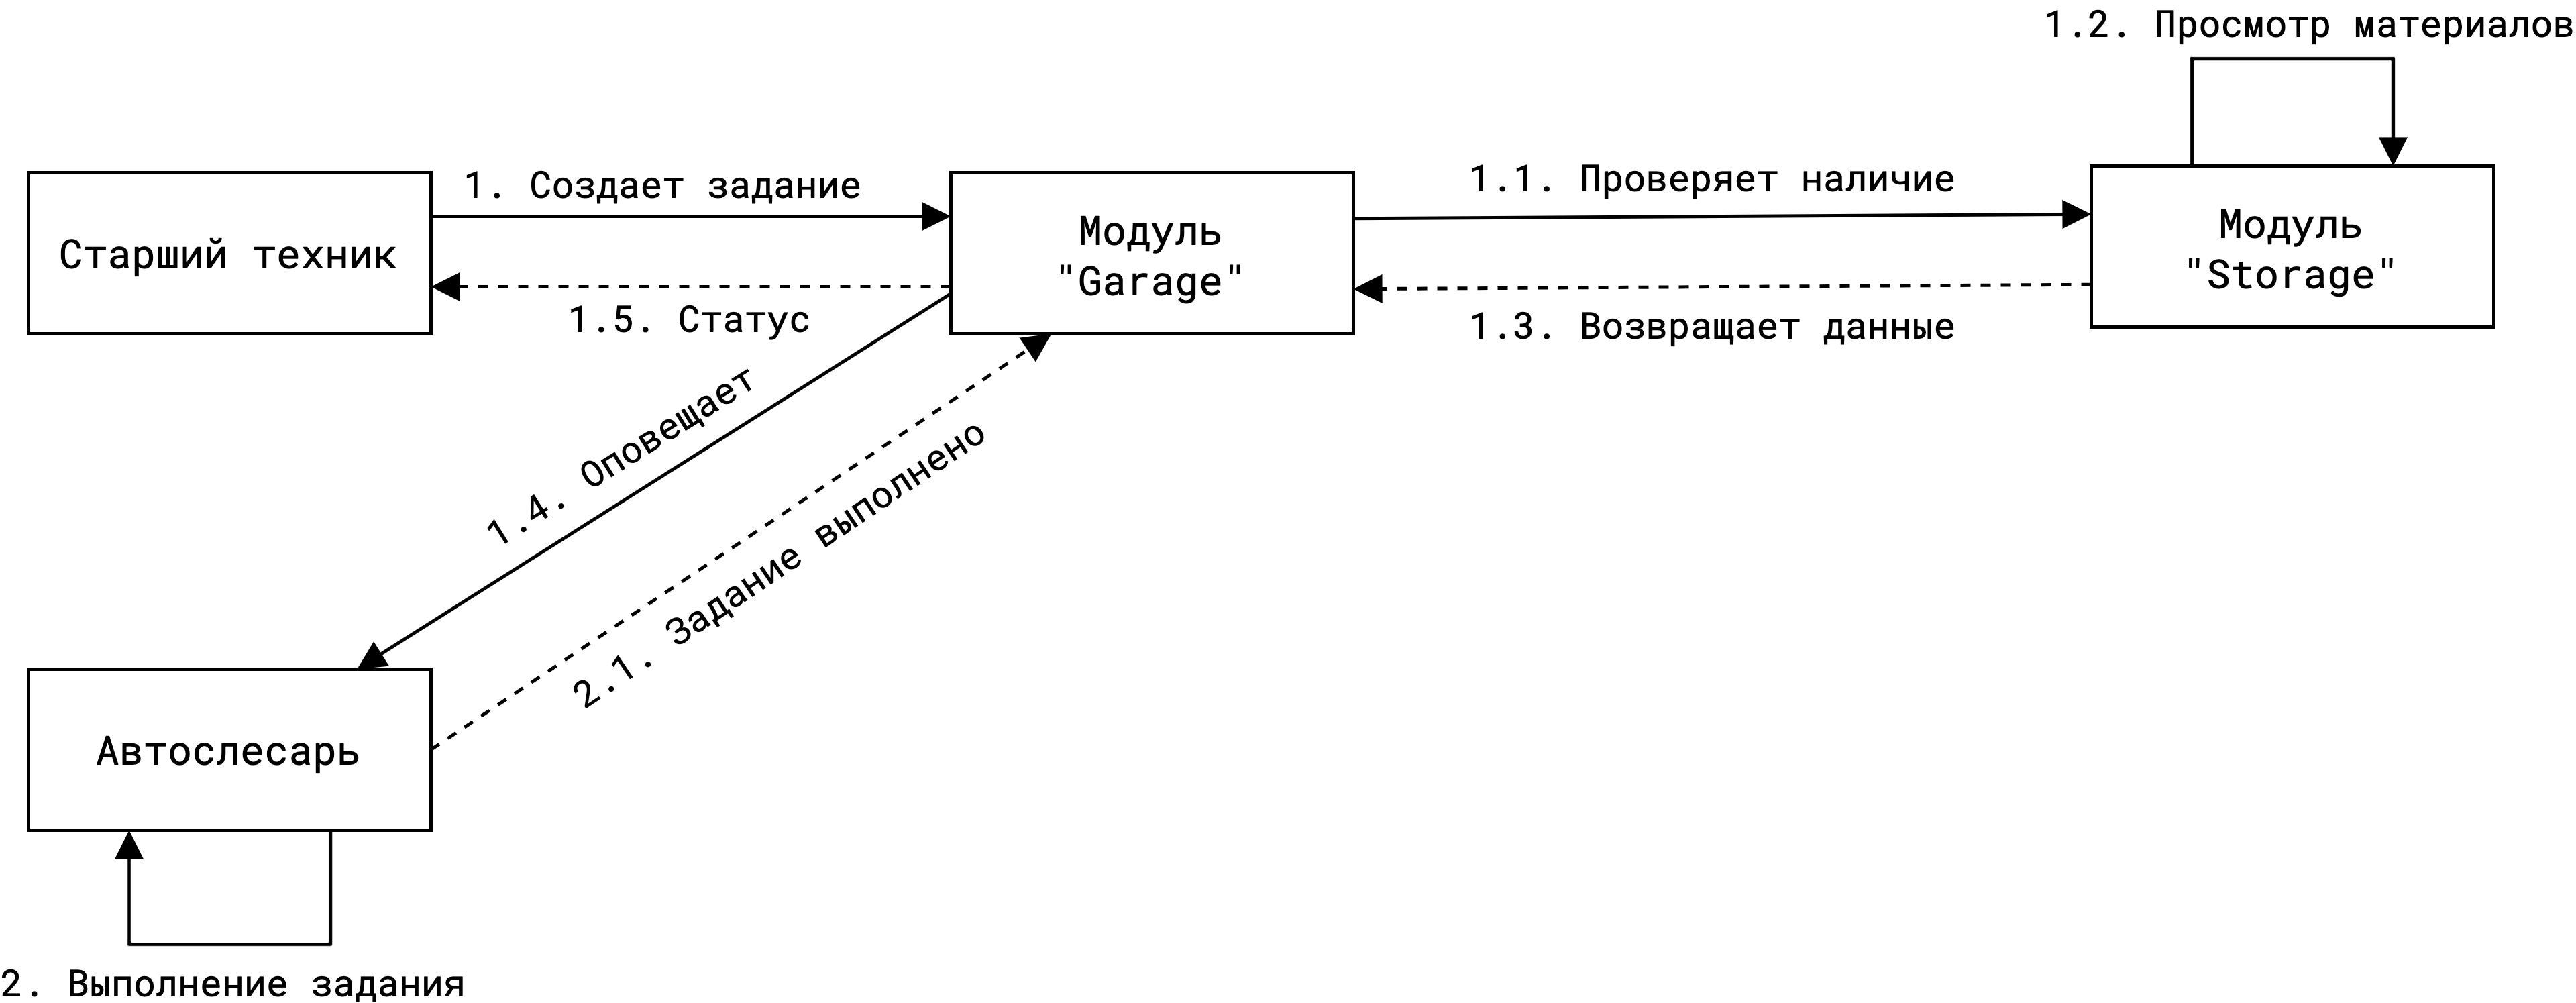
\includegraphics[keepaspectratio,width=\textwidth]{./images/aps.coursework-cooperation.png}
\caption{Диаграмма кооперации системы}
\label{fig:diag-caps.coursework-cooperation.pngooperation}
\end{figure}

Спецификация:

Старший техник создает задачу по техническому осмотру автомобиля. Модуль системы
\textquote{Garage} проверяет наличие материалов, необходимых для выполнения
работ, на складе. Модуль системы \textquote{Storage} просматривает наличие
материалов на складе и возвращает данные модулю \textquote{Garage}.

Модуль \textquote{Garage} оповещает автослесаря, назначенного на задание по
техническому осмотру автомобиля. Автослесарь выполняет необходимые работы и по
окончанию закрывает задачу. Модуль \textquote{Garage} оповещает старшего техника
о завершенной задаче.
